\documentclass[
  bibliography=totoc,     % Literatur im Inhaltsverzeichnis
  captions=tableheading,  % Tabellenüberschriften
  titlepage=firstiscover, % Titelseite ist Deckblatt
]{scrartcl}
\usepackage{scrhack}
\usepackage[aux]{rerunfilecheck}
\usepackage{fontspec}
\usepackage[ngerman]{babel}
\usepackage{graphicx}
\usepackage[section, below]{placeins}
\usepackage{caption}
\usepackage{scrlayer-scrpage}
%Mathe Pakete
\usepackage{amsmath}
\usepackage{amssymb}
\usepackage{mathtools}
\usepackage{xfrac}
\usepackage[math-style=ISO,bold-style=ISO,sans-style=italic,nabla=upright,partial=upright]{unicode-math}
\usepackage[
  math-style=ISO,
  bold-style=ISO,
  sans-style=italic,
  nabla=upright,
  partial=upright,
]{unicode-math}
\usepackage[
  locale=DE,
  separate-uncertainty=true,
  per-mode=symbol-or-fraction,
]{siunitx}
\usepackage{subcaption}
\usepackage{graphicx}
\usepackage{booktabs}
\usepackage{microtype}
\usepackage[unicode]{hyperref}
\usepackage{bookmark}
\setmathfont{Latin Modern Math}
\usepackage{csquotes}
\usepackage{wrapfig}
\usepackage[shortcuts]{extdash} % Trennung von Wörtern mit Strichen
\usepackage[backend=biber]{biblatex} %Literaturverzeichnis
\addbibresource{lit.bib}
\usepackage[section]{placeins}%Floats plazieren
\usepackage[version=4, math-greek=default,text-greek=default,]{mhchem} %Chemische Zeichen

\begin{document}
  \setlength{\parindent}{0em} %keine Einrückungen am Zeilenanfang
  \pagestyle{scrheadings}
  \clearpairofpagestyles
  \ofoot{\pagemark}

  \title{V105 \\Magnetische Momente}
  \author{Julian Hayduk \and Alex Nuss}
  \date{Durchführung: 13.12.2022, Abgabe: 20.12.2022}
  \subtitle{Versuchsort: TU Dortmund }
  \maketitle

  \thispagestyle{empty}
  \newpage
  
  \tableofcontents
  \thispagestyle{empty}
  \setcounter{page}{1}
  
  \newpage
  \section{Ziel des Versuches}
  Es soll das magnetische Moment eines Permamagneten über drei verschiedene Methoden bestimmt werden. 
  
  \section{Theorie}
  
  Neben Permamagneten können auch durch Strom durchflossenen Leiterschleifen Magnetfelder induziert werden, diese Magnetfelder werden charakteristisch durch das magnetische Moment 
  \begin{equation}
  \mu =I\cdot A
  \label{eqn:auswertung1}
  \end{equation}
  beschrieben, hierbei beschreibt $I$ den Strom durch die Leiterschleife mit der Querschnittsfläche $A$. Für einen Permamagneten ist die Berechnung kompliziert weswegen das 
  magnetische Moment experimentell über ein Drehmoment bestimmt wird. Das Drehmoment wird beschrieben durch: 
  \begin{equation}
    D_B=\vec{\mu} \times \vec{B}
    \label{eqn:moment}
    \end{equation}
    Aus \autoref{eqn:moment} folgt das auf den Dipol solange eine Drehmoment wirkt, bis das gesuchte magnetische Moment $\mu$ parallel zum Magnetfeld $B$ ist.
    Damit das erzeugte Magnetfeld möglichst homogen ist wird meistens ein Helmholtz-Spulenpaar verwendet. Das Spulenpaar besteht aus zwei in gleicher Richtung 
    durchflossenen meist kreisförmigen Spulen, welche so angeordnet sind, dass der Mittelpunkt auf einer Achse senkrecht zum Radialvektor liegt. Außerdem entspricht 
    der Abstand $d$ zwischen den einzelnen Spulen in etwa dem Spulenradius $R$. Somit kann das Magnetfeld auf der Symmetrieachse durch den Kreismittelpunkt als 
    homogen angesehen werden. Das Magnetfeld kann mit dem Biot-Savart-Gesetz berechnet werden
    \begin{equation*}
      dB=\frac{\mu_0I}{4\pi}\frac{\symup{d}\vec{s}\times \vec{r}}{r^3}
      \end{equation*}
      für $N$-Windungen folgt hier raus
      \begin{equation}
        B(x)=\frac{\mu_0I}{2}\frac{R^2}{(R^2+x^2)^\frac{3}{2}}\cdot e_r\cdot N
        \end{equation}
        Das Magnetfeld des Spulenpaars ergibt sich zu
        \begin{equation}
        B(0)=B_1(x)+B_1(-x)=\frac{\mu_0IR^2N}{(R^2+x^2)^\frac{3}{2}}
        \end{equation}
        
    \subsection{Bestimmung des magnetischen Moment über die Gravitation}
    Bei diesem Verfahren wird die Gravitationskraft 
        \begin{equation*}
          F_G=mg
        \end{equation*}
        zur Bestimmung des magnetischen Momentes verwendet. Die Masse $m$ im Abstand $r$ bewirkt dabei folgendes Drehmoment
        \begin{equation}
        D_G=m(\vec{r}\times \vec{g})
        \end{equation}
        Analog zu \autoref{eqn:moment} wird dieses minimal für $r$||$g$. Entgegengesetzt zu diesem Drehmoment wirkt das Magnetfeld des Helmholtz-Spulenpaars, 
        sodass ein Gleichgewichtszustand zwischen $D_G$ und $D_B$ nur bei einer bestimmten Magnetfeldstärke erreicht wird.
      
  \subsection{Bestimmung des magnetischen Moments über die Schwingungsdauer $T$}
  Um das magnetische Moment mithilfe der Schwingungsdauer zu bestimmen muss zunächst ein Körper so in Schwingung versetzt werden das seine Bewegung im 
  Magnetfeld einem harmonischen Oszilator entspricht. Eine solche Bewegung lässt sich durch folgende Gleichung beschreiben:
  \begin{equation}
  -|\mu_{Dipol}\times B|=J_K\frac{d^2\theta}{dt^2}
  \label{eqn:dgl}
  \end{equation}
  Die \autoref{eqn:dgl} wird durch die Schwingungsdauer $T$ gelöst. Unter Verwendung von
  \begin{equation}
  T^2=\frac{4\pi^2 J_K}{\mu_{Dipol}}\frac{1}{B}
  \label{eqn:auswertung2}
  \end{equation}
  lässt sich das magnetische Moment $\mu_{Dipol}$ über das Trägheitmoment $J_K$ des Körpers und der verwendeten Magnetfeldstärke B bestimmen.
  
  \subsection{Bestimmung des magnetischen Moments über die Präzession eines Magneten}
  \label{sec:Präzession}
  Wirkt eine äußere Kraft auf die Drehachse eines rotierenden Körpers, dann führt die Figurenachse eine Präzessionsbewegung aus.
  Die Präzessionsbewegung im Magnetfeld der Helmholtzspulen lässt sich durch die Differentialgleichung
  \begin{equation}
      \symbf{\mu_{Dipol}} \times \symbf{B} = \frac{d\symbf{L}_K}{dt}
  \end{equation}
  beschreiben, wobei die Präzessionsfrequenz $\Omega_p$
  \begin{equation}
      \Omega_p = \frac{\mu B}{|L_K|}
  \end{equation}
  eine Lösung der Differentailgleichung ist.
  Den Drehimpuls $L_K = J_K \omega$ der Kugel kann über das Trägheitsmoment $J_K$ der Billiardkugel und deren Kreisfrequenz $\omega = 2\pi \nu$ bestimmt werden.
  Da sich die Präzessionsfrequenz $\Omega_p$ aus der Zeit $T_p$ für einen Umlauf berechnen lässt, lässßt sich das magnetische Moment $\mu_{Dipol}$ der Kugel über
  \begin{equation}
      \frac{1}{T_p} = \frac{\symbf{\mu}_{Dipol}}{2 \pi L_K} B
      \label{eqn:praezession}
  \end{equation}
  berechnen.\\

  Durch ein Stroboskop wird die notwendige Konstanz der Rotationsfrequenz $\nu = \omega / 2 \pi$ kontrolliert.
  Wenn die weiße Markierung auf der Kugel stationär unter dem Stroboskop erscheint, dann hat die Kugel die am Gerät eigenstellte Frequenz.
  Da die Frequenz exponentiell mit der Zeit abnimmt, muss direkt nach dem Erreichen der eingestellten Frequenz mit der Messung begonnen und
  eine geeignete Frequenz gewählt werden, zwischen $\nu = \SI{4}{\Hz}$ und $\nu = \SI{6}{\Hz}$, weil hier der Abfall der Exponentialkurve bereits hinreichend langsam geschieht (etwa 2 Hz pro Minute).
  
  \section{Durchführung}
  \subsection{Aufbau}
    Zur Erzeugung des äußeren Magnetfeldes wird ein Helmholz-Spulenpaar verwendet welches folgende Parameter besitzt: Windungen $N=195$, 
    Abstand der Spulen zueinander $d=0.138m$ und Spulenradius $R=0.109m$. In der Mitte dieses Spulenpaares befindet sich ein Messingpodest auf dem sich
    eine Kugel der Masse $m_K = 141.65\,\si{\gram}$ und mit eingegossenem Permamagneten befindet. Das Podest ist mit einem Kompressor verbunden welcher ein Luftkissen erzeugt wodurch die Kugel 
    Näherungsweise Reibungsfrei auf dem Podest liegt. Der in der Kugel befindliche Permamagnet ist so ausgerichtet das sein magnetisches Moment in Richtung 
    eines auf der Kugel befindlichen Stieles zeigt. Die Spulen sowie das Luftkissen werden über ein externes Steuergerät bedient.
 
  \subsection{Bestimmung über Gravitation}
    Die Aluminiumstange mit der verstellbaren Masse wird in die Kugel gesteckt,
    die auf dem Messingzylinder platziert wird.
    Am Steuergerät wird das Luftkissen eingeschaltet und die Feldrichtung auf \enquote{up} und
    der Feldgradient auf \enquote{off} gestellt.
    Für einen vorher festgelegten Abstand $r$ der Hebelmasse wird das $\symbf{B}$-Feld über
    die Stromstärke $I$ so reguliert, dass sich die Kugel im Gleichgewicht befindet.
    Die Werte für $r$ und $I$ werden notiert und die Messung für verschiedene Abstände $r$ wiederholt.
    
  \subsection{Bestimmung über Schwingungsdauer}
    
    Die vorherigen Einstellungen am Steuergerät werden beibehalten.
    Es werden 10 Messungen für unterschiedliche Magentfeldstärken $\symbf{B}$ durchgeführt.
    Die Kugel wird um einen kleinen Winkel ausgelenkt, sodass sie wie ein harmonischer Oszillator schwinkt.
    Anschließend werden 10 Periodendauern $T$ am Stück gemessen und das Ergebnis gemittlet.
    
  \subsection{Bestimmung über Präzession}
    
    Am Steuergerät wird jetzt noch zusätlich das Stroboskop mit einer Frequenz von 5,5 Hertz eingeschaltet.
    Die Kugel wird in eine möglichst stabile Rotation versetzt, um später eine ungewollte Nutation zu vermeiden.
    Dabei soll die Drehachse nicht vertikal sein.
    Mit Hilfe des Stroboskops wird die Frequenz der Kugel eingestellt.
    Wenn der weiße Punkt auf der Kugel stationär erscheint, stimmt die Frequenz mit der des Stroboskops überein.
    Jetzt wird das Magentfeld eingeschaltet und die Kugel beginnt zu präzedieren.
    Es wird die Zeit $T$ von 3 Umläufen gemessen und die mittlere Umlaufzeit gebildet.
    Die Messung wird durchgeführt mit 10 verschiedenen Magnetfeldstärken $\symbf{B}$.


  \newpage
  \section{Auswertung}
  \subsection{Bestimmung über Gravitation}
  \begin{table}[h]
    \centering
    
    
    \begin{tabular}{c c c}
      Abstand Gewicht zum Stiel$\,/\,\si{\centi\meter}$ & Stromstärke$\,/\,\si{\ampere}$ & Magnetfeldstärke$\,/\,\si{\milli\tesla}$ \\
      \toprule
          4.0 & 1.1 & 1.4917\\
          4.5 & 1.2 & 1.6273\\
          5.0 & 1.3 & 1.7629\\
          5.5 & 1.4 & 1.8985\\
          6.0 & 1.5 & 2.0341\\
          6.5 & 1.6 & 2.1698\\
          7.0 & 1.7 & 2.3054\\
          7.5 & 1.8 & 2.4410\\
          8.0 & 1.9 & 2.5766\\
          8.5 & 2.0 & 2.7122\\
      \bottomrule
    \end{tabular}
    \caption{Messdaten zur Bestimmung über die Gravitation}
    \label{tab:some_data1}
  \end{table}
  \begin{wrapfigure}{r}{6.5cm}
    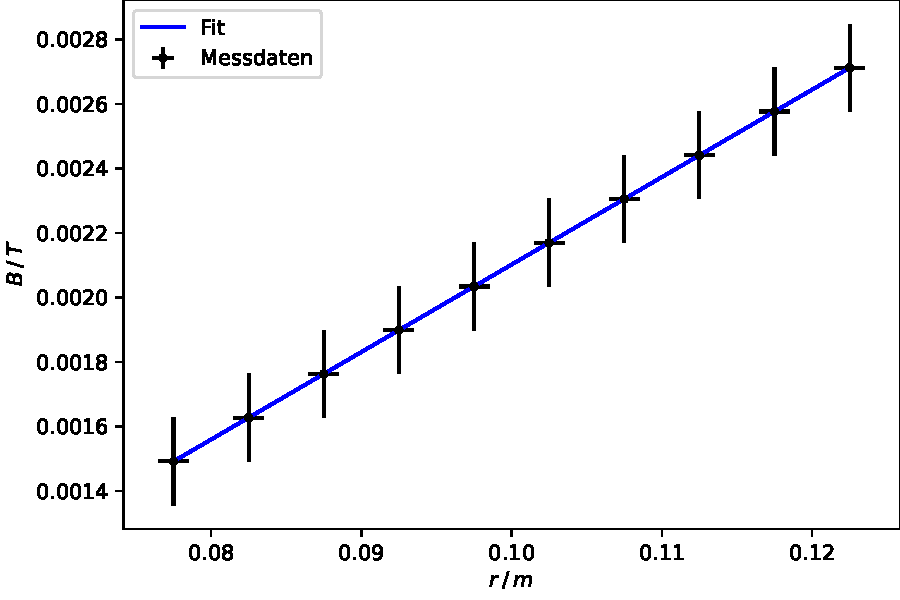
\includegraphics[scale=.6]{plot1.pdf.pdf}
    \caption{Plot zur Bestimmung über Gravitation}
    \label{fig:Plot_1}
  \end{wrapfigure}
  Durch umschreiben von \autoref{eqn:auswertung1} zu
  \begin{equation}
  \mu_{Dipol}=\frac{mrg}{B}
  \end{equation}
  mit m als Masse, g der Erdbeschleunigung \\und $\frac{r}{B}$ als Steigung der Ausgleichsgraden\\ ergibt sich für das magnetische Moment.\\
  In der \autoref{tab:some_data1} sind die Messdaten und die ausgerechneten Magnetfeldstärken des Spulenpaares zu finden. In der \autoref{fig:Plot_1} wird das Magnetfeld B 
  gegen den Abstand des Gewichts zum Stiel der Kugel aufgetragen. Die Ausgleichsgrade wird mittels Python berechnet und ergibt für die Parameter :
  Gleichung \eqref{eqn:auswertung1} lässt sich dann zu umstellen und das magnetsiche Moment kann berechnet werden:
  \begin{equation*}
    \symbf{\mu}_{Dipol} = (0,501 \pm 0,008) \: \text{A}^{2}/\text{m}
  \end{equation*}

  \newpage
  \subsection{Bestimmung über Periodendauer}
  \begin{table}[h]
    \centering
   
    
    \begin{tabular}{c c c c}
      Stromstärke$\,/\,\si{\ampere}$  & Magnetfeldstärke$\,/\,\si{\milli\tesla}$ & Dauer von 10 Perioden$\,/\,\si{\ampere}$ & Gemittelte Periodendauer$\,/\,\si{\ampere}$ \\
      \toprule
      1.5 & 2.0341 & 13.2 & 1.320 \\
      1.7 & 2.3054 & 11.23 & 1.123 \\
      1.9 & 2.5766 & 10.43 & 1.043 \\
      2.1 & 2.8478 & 9.56 & 0.956 \\
      2.3 & 3.1190 & 9.47 & 0.947 \\
      2.5 & 3.3902 & 8.96 & 0.896 \\
      2.7 & 3.6614 & 8.3 & 0.830 \\
      2.9 & 3.9327 & 8.16 & 0.816 \\
      3.1 & 4.2039 & 8.21 & 0.821 \\
      3.3 & 4.4751 & 7.7 & 0.770 \\
      3.5 & 4.7463 & 7.6 & 0.760 \\
      \bottomrule
    \end{tabular}
    \caption{Messdaten zur Bestimmung über die Periodendauer}
    \label{tab:some_data2}
  \end{table}
  \FloatBarrier
  \begin{wrapfigure}{r}{6.5cm}
    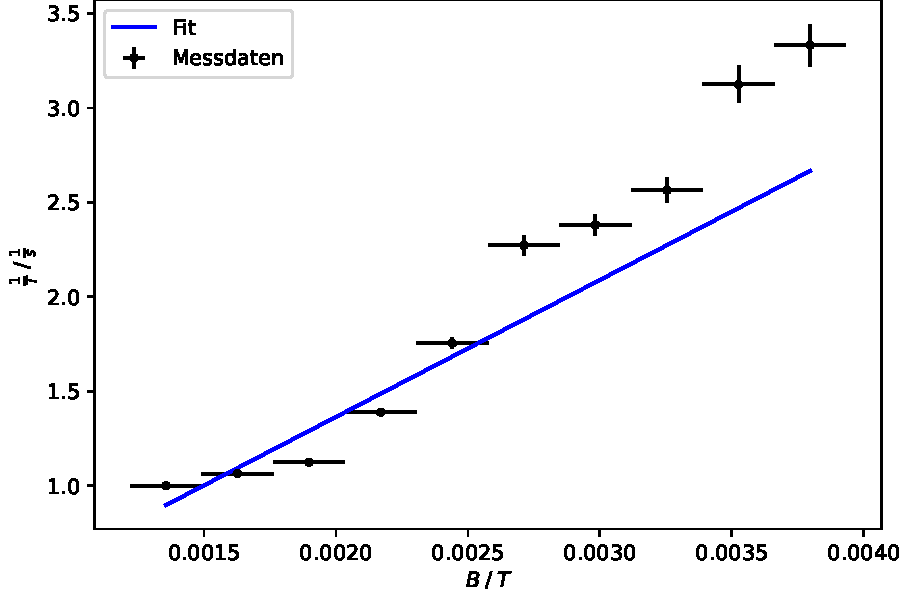
\includegraphics[scale=.6]{plot3.pdf}
    \caption{Plot zur Bestimmung über die Periodendauer}
    \label{fig:Plot_2}
  \end{wrapfigure}
  \FloatBarrier
  In der \autoref{tab:some_data2} sind die Messdaten und die ausgerechneten Magnetfeldstärken des Spulenpaares sowie die gemittelte Schwingungsdauer zu finden. 
  In der \autoref{fig:Plot_1} wird die quadrierte Schwingungsdauer $T^2$ gegen den Kehrwert des Magnetfeldes geplotet. Die Ausgleichsgrade wurde mittels Python berechnet. 

  Gleichung \eqref{eqn:auswertung2} lässt sich dann umstellen zu
  \begin{equation}
    \symbf{\mu}_{Dipol} = 4 \pi^2 J_K \frac{1}{a}
  \end{equation}
  mit $a = T^{2} \cdot B$.
  Das magnetische Moment lässt sich dann einfach berechnen:
  \begin{equation*}
    \symbf{\mu}_{Dipol} = (0,281 \pm 0,018) \: \text{A}^{2}/\text{m}
  \end{equation*}

  \subsection{Bestimmung über Präzession}
  \begin{table}[h]
    \centering
   
    
    \begin{tabular}{c c c }
      Stromstärke$\,/\,\si{\ampere}$  & Magnetfeldstärke$\,/\,\si{\milli\tesla}$ & Gemittelte Periodendauer$\,/\,\si{\ampere}$ \\
      \toprule
      1.5 & 2.0341 &  \\
      1.7 & 2.3054 &  \\
      1.9 & 2.5766 &  \\
      2.1 & 2.8478 &  \\
      2.3 & 3.1190 &  \\
      2.5 & 3.3902 &  \\
      2.7 & 3.6614 &  \\
      2.9 & 3.9327 &  \\
      3.1 & 4.2039 &  \\
      3.3 & 4.4751 &  \\
      3.5 & 4.7463 &  \\
      \bottomrule
    \end{tabular}
    \caption{Messdaten zur Bestimmung über die Präzession}
    \label{tab:some_data3}
  \end{table}
  \FloatBarrier
  \begin{wrapfigure}{r}{6.5cm}
    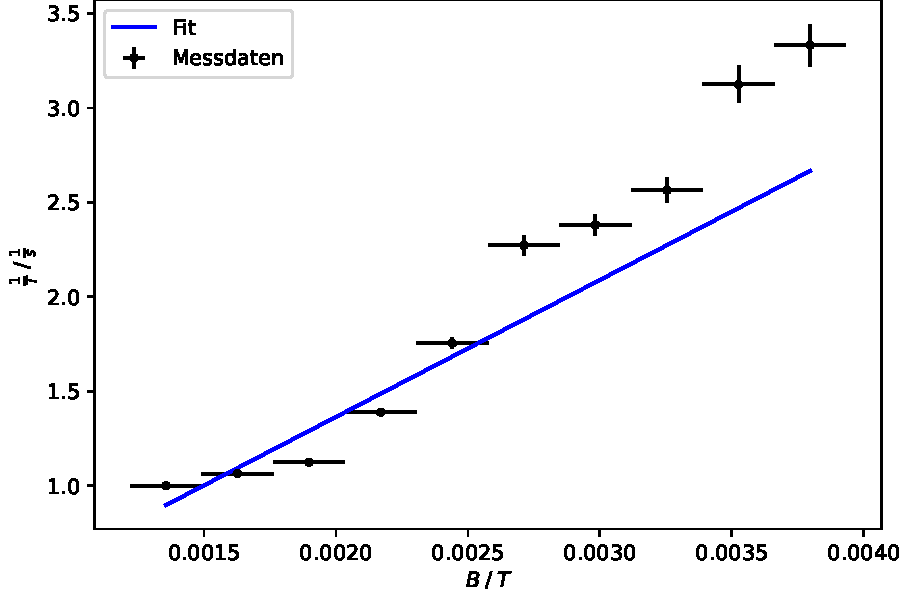
\includegraphics[scale=.6]{plot3.pdf}
    \caption{Plot zur Bestimmung über die Präzession}
    \label{fig:Plot_3}
  \end{wrapfigure}
  \FloatBarrier
  In der \autoref{tab:some_data3} sind die Messdaten zu finden. 
  In der \autoref{fig:Plot_3} wird $B$ gegen $1/T$ aufgetragen. Die Ausgleichsgrade wurde mittels Python berechnet. 
  Um das magnetische Moment bestimmen zu können muss jetzt noch Gleichung \eqref{eqn:praezession} umgeformt werden
  \begin{equation}
    \symbf{\mu}_{Dipol} = 2 \pi L_K a
  \end{equation}
  mit $a = 1/(T \cdot B)$ und $L_K = J_K \omega$.
  Das letzte Verfahren liefert dann für das magnetische Moment den Wert:
  \begin{equation*}
    \symbf{\mu}_{Dipol} = (0,86 \pm 0,03) \: \text{A}^{2}/\text{m}
  \end{equation*}
  
  \newpage
  \section{Diskussion}
  \begin{table}[h]
    \centering
    \begin{tabular}{c c}
       Messmethode & Experementelles Ergebnis für $\mu_{Dipol}$\\
      \toprule
         Gravitation & $0.5\,\si{\ampere\meter^2}$ \\
         Periodendauer & $0.28\,\si{\ampere\meter^2}$ \\
         Präzession & $ 0.86\,\si{\ampere\meter^2}$\\
      \bottomrule
    \end{tabular}
    \caption{Messergebnisse}
  \end{table}




  \newpage
  \section{Literaturverzeichnis}
  [1] TU Dortmund. V105: Magnetische Momente. 2022.
\end{document}
